\section{Introduction}
\todo{Adjust to be more benchmarky}
Emerging web applications increasingly rely on decentralized architectures to give users control over their personal data.
Structured decentralized ecosystems, such as Solid~\cite{sambra2016solid} and Mastodon~\cite{raman2019challenges},
encourage users to keep their data in small, independent stores following shared data models.
This paradigm shift is increasingly vital for automated systems, such as LLM-based AI agents,
which query these decentralized structures to extract facts for task performance or question answering~\cite{walter2025grasp,karki2026agentic,bernerslee2017charlie}.
While this approach strengthens user autonomy, the absence of a central data authority naturally creates a highly multi-perspective environment. 
Data spreads across thousands of heterogeneous sources that frequently contain overlapping, diverse, 
or potentially conflicting claims.
Query engines must therefore dynamically fetch and integrate this information at runtime~\cite{taelman_sigweb_queryengineshypermedia_2024}, 
not only to discover conflicting statements and multiple perspectives, 
but to reconcile these claims to provide a coherent answer to the user or agent.

Traditional federated querying approaches~\cite{schwarte2011fedx,schmidt2011fedbench,heling2022federated} support the integration of decentralized data sources,
but they typically assume a small (10-100) set of well-described and consistently available endpoints~\cite{dang2023fedshop}. 
These assumptions fail once data is spread across thousands of small units that enforce local access-control policies.
In addition, enforcing fine-grained access control policies~\cite{esteves2021odrl} on large sources with expressive interfaces introduces notable 
overhead~\cite{padia2015attribute}, making standard approaches unsuitable for highly decentralized environments.

Newer decentralized environments, such as Solid, often expose data as lightweight HTTP resources instead of highly expressive query interfaces. 
Many of these resources are not known in advance and can only be discovered during query execution. 
While their simplicity lowers the cost of enforcing fine-grained controls,
this setting requires a federation model that can operate over a very large number of small sources,
many of which may be encountered at runtime, without relying on prior aggregation.
Traditional federated approaches are insufficient in this setting due to the assumption of a small number of large endpoints.
Additionally, these approaches often assume prior knowledge of the sources, which is not feasible in decentralized environments where discovery is a key requirement.
Executing SPARQL queries using Link Traversal-based Query Processing (LTQP)~\cite{hartig2009executing} fits these needs.
It discovers documents incrementally by following URIs encountered during execution, 
starting from an initial set of seed documents provided by either the user or the query.
Its link-driven, asynchronous traversal supports fine-grained permissions 
and allows systems to discover without knowing the location of all decentralized data sources beforehand.

However, the fact that LTQP discovers documents incrementally creates significant challenges for efficient execution. 
Using the traditional optimize-then-execute query processing paradigm is difficult, as the query itself determines which data will be accessed. 
As a result, the optimizer has no prior knowledge of the relevant data until the query’s traversal has already begun.
Some approaches optimize query execution without prior knowledge by using zero-knowledge query planning~\cite{hartig2011zero} or adaptive query processing~\cite{hanski2025link}. 
These yield modest but inconsistent performance gains, depending on the decentralized environment and the heuristics used~\cite{taelman2023link}.
However, other aspects of zero-knowledge LTQP optimization, such as link prioritization~\cite{hartig2016walking},
are unlikely to improve query result arrival times in emerging decentralized environments~\cite{eschauzier2025revisiting}.

Consequently, other works explore using precomputed server-side information as prior knowledge 
or relevance indexes to efficiently execute LTQP queries \newline \cite{tam2024opportunities,umbrich2011comparing,hanski2024observations}.
While these approaches offer greater performance benefits, they require the server to maintain these indexes.
This raises the cost of serving resources and complicates privacy and access control.

To avoid server-side overhead, engines can derive prior knowledge directly on the client.
In decentralized settings, LTQP operates inherently client-side, with a single engine instance serving one or more applications,
often specific to a particular user.
As these users and thus the used applications issue sequences of correlated queries,
the engine identifies frequently accessed data and its characteristics.
This allows engines to implement \emph{personalized} query optimization algorithms 
that leverage local access patterns to build necessary prior knowledge.


\begin{figure}
	\centering
	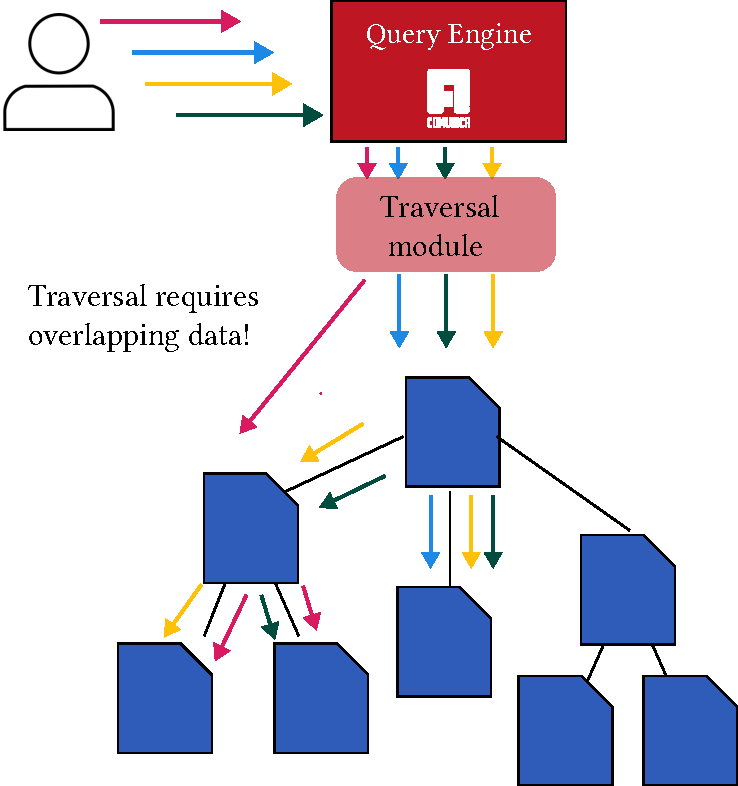
\includegraphics[width=.9\columnwidth]{figures/overlapping_queries_fixed.pdf}
	\caption{When users interact with query engines, their queries intentions and thus relevant data to the query can overlap, leading to opportunities for personalized optimization.}
	\label{fig:intro-overlap}
\end{figure}

Benchmarking these approaches requires realistic query sequences.
Traditional benchmarks (e.g., WatDiv~\cite{alucc2014diversified}, \\ BSBM~\cite{bizer2011berlin}, LargeRDFBench~\cite{saleem2018largerdfbench})
execute isolated or repeated query templates, which fails to capture client-side dynamics accurately. 
Furthermore, while centralized SPARQL optimization relies on
real query logs~\cite{berendt2013usewod2013,picalausa_what_2011,bonifati_darql_2018,stadler2024lsq}, 
such logs do not yet exist for decentralized LTQP environments. 
Consequently, we need a standardized benchmark that realistically simulates user query sequences 
to prevent fragmented evaluation practices.

In this paper, we address this gap by introducing SolidSessionBench,
a benchmark extending SolidBench~\cite{taelman2023link} to generate realistic query sequences.
These sequences capture usage patterns identified in social network literature, 
a domain naturally rich in multi-perspective data, 
alongside patterns observed in real-world SPARQL logs.

To evaluate the realism of our generated query sequences without access to real-world query logs, 
we investigate four baseline client-side caching strategies combined with two cardinality estimatoin techniques
in the Comunica LTQP engine~\cite{taelman2018comunica,taelman2023link}. 
We use these simple algorithms to establish a performance baseline and demonstrate the necessity of sequence-based evaluation.
Comparing this baseline against existing literature shows 
that current evaluation techniques are insufficient for client-side caching in LTQP.

By enabling researchers to evaluate personalized query optimization against actual user behaviors,
SolidSessionBench lays the foundation for performant client-side querying. 
Ultimately, efficient LTQP execution over decentralized sources facilitates the rapid identification of conflicting information
and the application of consistency fixes across multi-dimensional knowledge graphs.

In summary, this paper makes the following contributions:
\begin{itemize}
    \item We review empirical usage patterns in web and query-based systems
    to establish a foundation for realistic sequence simulation.
    
    \item We propose a simulation methodology based on the literature review
	 that models logical query sessions,
    user interest-driven data locality, and dynamic query refinements
    mapped to query engine choke points.
    
    \item We introduce SolidSessionBench, a fully configurable benchmark
    integrating this methodology to evaluate client-side query optimization
    under realistic conditions.
    
    \item We implement four baseline client-side caching strategies
    for Link Traversal Query Processing (LTQP),
    alongside two cache-based cardinality estimation techniques.
    
    \item We evaluate these strategies, demonstrating that realistic query sequences
    reveal critical performance dynamics that traditional benchmarking approaches miss.
\end{itemize}


This article extends our previous work presented at the International Semantic Web Conference 
(ISWC) 2026~\cite{eschauzier2026solidsessionbench}. 
While the initial study introduced the SolidSessionBench methodology and evaluated standard in-memory caching strategies, 
this version expands both the technical implementations and the experimental analysis. 

Specifically, we introduce in-memory and disk-based quad store caches to unify cached triple indexes. 
Furthermore, we enhance the original cache-based cardinality estimation technique
by incorporating reachability to generate more accurate estimates. 
Finally, we expand the experimental analysis by applying a linear mixed-effects regression model to quantify
the performance impact of individual query execution choke points. 

Beyond expanded explanations and examples, this extended version provides a thorough investigation of diverse cache implementations. 
Overall, we place a stronger focus on cache performance, the implications of our findings, 
and concrete directions for future research.

The remainder of this paper is structured as follows.
Section~\ref{sec:related-work} reviews prior benchmarking approaches and real-world query usage patterns.
Section~\ref{sec:simulation-methodology} outlines our simulation methodology and defines the resulting hyperparameters.
Section~\ref{sec:client-side-caching} introduces the technical mechanics of client-side caching strategies in LTQP.
Section~\ref{sec:evaluation} evaluates the benchmark using proxy measures of realism. 
Finally, Section~\ref{sec:conclusion} concludes the paper and presents a plan for benchmark sustainability.

